\input{style/settings}
\input{style/short_commands}
\pagestyle{fancy}
\fancyhf{}
\fancyhead[R]{página\;\thepage/\pageref{LastPage}}
\fancyhead[L]{Osvaldo Uriel Calderón Dorantes}
\fancyfoot[L]{Imagenología Biomédica}
\fancyfoot[R]{Facultad de Ciencias, UNAM 
\includegraphics[scale=0.13]{style/Sheikah.pdf}}
\fancypagestyle{plain}{
  \fancyfoot[C]{}
}
\makeatletter
\def\@seccntformat#1{%
  \expandafter\ifx\csname c@#1\endcsname\c@section\else
  \csname the#1\endcsname\quad
  \fi}
\makeatother
%%%%%%%%%%%%%%%%%%%%%%%%%%%%%%%%%%%%%%%%%%%%%%%%%%%%%%%
%%%%%%%%%%%%%%%%%%%%%%%%%%%%%%%%%%%%%%%%%%%%%%%%%%%%%%%%%%%
\begin{document}
\begin{flushleft}
Osvaldo Uriel Calderón Dorantes, \hfill Imagenología Biomédica\\
316005171 \hfill osvaldo13576@ciencias.unam  \\
Facultad de Ciencias\\
\underline{Universidad Nacional Autónoma de México}
\end{flushleft}

\begin{flushright}\vspace{-5mm}

\includegraphics[height=1.5cm]{style/logo.pdf}
\end{flushright}
 
\begin{center}\vspace{-1cm}
\textbf{ \large \customfont{Tarea EXAMEN\\
Módulo MEDICINA NUCLEAR}}\\
\today
\end{center}
%\medskip\hrule\medskip
%%%%%%%%%%%%%%%%%%%%%%%%%%%%%%%%%%%%%%%%%%%%%%%%
%{\small \textbf{Nota: A las unidades las pondré dentro de corchetes \ec{[\tx{unidad}]} para no confundir entre variables y realizar el análisis dimensional fácilmente.}}
\medskip\hrule\bigskip

\newlength{\strutheight}
\settoheight{\strutheight}{\strut}


\textbf{Parte teórica}: Investigue (citando fuentes) o explique con base en lo visto en clase la respuesta a las siguientes preguntas, sea conciso:

\begin{enumerate}[1.]
  \item Explique en 10 renglones (máximo) el funcionamiento del generador de \ec{^{99m}}Tc.
  
  \begin{figure}[!ht]
    \centering
    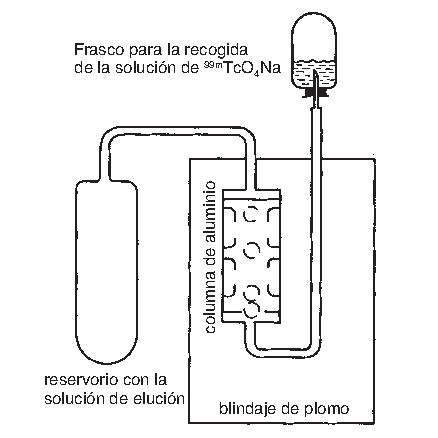
\includegraphics[width=0.5\textwidth]{./figuras/tc_gen.pdf}
    \caption{Diagrama de un generador de \ec{^{99m}}Tc. La figura se recuperó de \citet{andre}.}
    \label{p1:tc_gen}
    \end{figure}


El generador emplea el radionúclido de \ec{^{99}}Mo para producir \ec{^{99m}}Tc que emite fotones gamma de energía de \ec{140\un{MeV}}.  En la figura \ref{p1:tc_gen} se describe el proceso, del ion de molibdato MoO\ec{_4^{2-}} se obtiene el pertecnetato \ec{^{99m}}TcO\ec{_4^{-}} a partir del eluyente salino. La separación o \textit{lavado} se da gracias a que los iones de molibdato quedan adheridos a una columna de alúmina Al\ec{_2}O\ec{_3} ya que no es soluble en solución salina, entonces cuando se requiere el \ec{^{99m}}Tc se agrega solución salina al generador se obtiene este tecnecio metaestable como pertecnetato de sodio \ec{^{99m}}TcO\ec{_4}Na \citep{guy,IM}.







  \item Explique en 10 renglones (máximo) el método de reconstrucción iterativa mencionando sus ventajas sobre la retroproyección filtrada para estudios SPECT.
  
El método de reconstrucción iterativa consiste en realizar una estimación inicial de la distribución de actividad del objeto a estudiar, luego, se calcula la proyección estimada proyectando hacia adelante o reproyección. Entones, según la comparación entre las proyecciones medidas y estimadas, la estimación inicial se ajusta de acuerdo a un criterio el cual deberá converger a la solución deseada, así que este proceso de reproyectar, comparar, retroproyectar y ajustar se repite hasta que la estimación se ajusta a la solución deseada \citep{smith}. Las ventajas con respecto a la retroproyección filtrada es que se obtiene una imagen con bajo ruido, se eliminan los artefactos de estrella, además en caso de tener datos faltantes el algoritmo sigue cumpliendo su función de reconstrucción de imagen \citep{smith,IM}.




\pagebreak





  \item Investigue y explique 2 aplicaciones clínicas de las siguientes técnicas de Medicina Nuclear, 5   renglones máximo por aplicación:
  \begin{enumerate}[a.]
    \item Gammagrafía.
    \begin{itemize}
      \item \textbf{Primera aplicación.} Estudio de gammagrafía ósea para el estudio morfofuncional del esqueleto que se basa en la distribución del radiotrazador en la matriz mineral ósea, estudios de los cuales se puede determinar la ubicación de tumores primarios o secundarios por metástasis \citep{app1}.
      


      \item \textbf{Segunda aplicación.} Aplicación de gammagrafía de perfusión miocárdica que se emplea para el estudio del flujo sanguíneo regional coronario para el diagnóstico y pronóstico de la enfermedad coronaria  \citep{app2}.
    \end{itemize}
    \item SPECT.
    \begin{itemize}
      \item \textbf{Primera aplicación.} Se usa en el estudio de perfusión cerebral, el cual el metabolismo regional está relacionado con el flujo sanguíneo regional en donde se usan compuestos marcados con \ec{^{99m}}Tc, \ec{^{99m}}Tc-hexa-\linebreak metilpropilen-amina-oxima (HMPAO) o \ec{^{99m}}Tc-etinilescisteinato-dímero (ECD). Las imágenes obtenidas en este estudio se emplean definir el estado patológico y neurológico de un paciente \citep{app34}.
      \item \textbf{Segunda aplicación.} Se emplea para la identificación de tumores neuroendocrinos desarrolladas a partir de células neuroendocrinas de pulmones, páncreas,  timo y glándulas suprarrenales empleando el radiotrazador \ec{^{111}}In en  \ec{^{111}}In-octreotido y el \ec{^{111}}In-pentetreotido \citep{app34}.
    \end{itemize}
    \item PET.
    \begin{itemize}
      \item \textbf{Primera aplicación.} Empleando la timidina de \ec{^{11}}C y la fluorotimidina \ec{^{18}}F  (FLT) es posible realizar estudios de proliferación celular cuyo interés clínico es la estadificación de cáncer de pulmón, evaluación de cáncer de cerebro y predictor de la respuesta tumoral \citep{app56}.
      \item \textbf{Segunda aplicación.} En oncología, específicamente en el cáncer de carcinoma de colon primario, se emplea esta técnica para detectar esta neoplasia con una sensibilidad del \ec{90\%} contra el \ec{60\%} de la CT en estadios tempranos  \citep{app56}.
    \end{itemize}
  \end{enumerate}
  \item ¿Cómo se define y para qué se usa el valor SUV (Standardized uptake value)?
  

El valor SUV se define como se establece en la ecuación \ref{e:1} \citep{SUV2}:
\eq{e:1}{SUV=\dfrac{r}{\p{a'/w}}}

donde \ec{r} es la concentración de actividad radiactiva en unidades \ec{\un{kBq/ml}} que es medida por el escáner PET dentro de una región de interés (ROI), \ec{a'} es la cantidad de FDG inyectada y corregida debido a descomposición cuyas unidades son \ec{\un{kBq}} y \ec{w} es el pase del paciente en unidades \ec{\un{g}}, el cual se considera como sustituto de un volumen de distribución del trazador \citep{SUV2}. 


Este valor es una medida semicuantitativa referente a la captación del tejido  y se ha empleado para entre niveles de captación ``normales'' y ``anormales''.  Para el hígado normal se tiene el rango \ec{2<SUV<5}, observemos que esta cantidad se considera adimensional ya que se hace la suposición que \ec{1\un{ml}} de tejido pesa \ec{1\un{g}} \citep{SUV1,SUV2}. Sin embargo, se toman en cuenta los factores que afectan al SUV y son la precisión en la calibración de la dosis, el tiempo pasado entre la inyección del radiofármaco y la toma de la imagen, peso del paciente, artefactos debido al movimiento y los niveles de glucosa en sangre del paciente \citep{SUV3}.




  \item ¿Cómo afecta el alcance del positrón en la calidad de imagen en PET?

Recordemos que el alcance del positrón es la distancia entre el átomo emisor del positrón y del evento de aniquilación, independientemente de la trayectoria tomada por el positrón, el cual toma valores entre \ec{0.2} a \ec{2.0\un{mm}} según la energía cinética del radionúclido. De este parámetro físico, el cual depende de su energía máxima y en el medio en que se propagan, junto con otros e instrumentales definen \ec{FWHM} (Full Width at Half Maximum) que es la anchura a media altura el cual caracteriza la resolución espacial del sistema PET, el cual toma un valor de \ec{0.1} a \ec{2.5\un{mm}} según el diámetro del anillo de detectores del escáner  \citep{cherry,range_posi}. Por lo tanto, un aumento en el alcance del positrón proporciona un aumento en el valor \ec{FWHM} y se tendrá una degradación en la calidad de imagen.


\pagebreak

  \item Describa 2 factores influyen en la resolución espacial y en el contraste de las imágenes de MN. Dos factores por parámetro, 5 renglones máx. por parámetro.
  

\begin{enumerate}[a.]
  \item Resolución espacial.
  \begin{itemize}
    \item \textbf{Primer factor}. En el colimador, la resolución espacial es dependiente de la geometría del colimador y en la pérdida de resolución es debido a un aumento entre la distancia fuente-colimador \citep{IM}. 
    \item \textbf{Segundo factor}. En el sistema de detección, pueden ocurrir efectos físicos (dispersión múltiple) de los rayos gamma en donde dos tubos fotomultiplicadores registren un solo evento \citep{IM}.
  \end{itemize}
  \item Contraste.
  \begin{itemize}
    \item \textbf{Primer factor}. Un primer factor es la dispersión que ocurre dentro del paciente en donde los fotones llegan al sistema de detección con una linea de respuesta errónea \citep{IM}.
    \item \textbf{Segundo factor}. En los sistema de imágenes de gamma cámara, el contraste se ve afectado por la penetración septal en donde ocurra una atenuación incompleta debido a las paredes delgadas del colimador permitiendo que el fotón ingrese al sistema de detección con una línea de respuesta errónea (la trayectoria del fotón no es paralela a las paredes del colimador)  \citep{IM}.
  \end{itemize}
\end{enumerate}







  \item ¿Qué es el efecto de volumen parcial en Medicina Nuclear?
  
Es un artefacto que es causado por la mezcla de tejidos con diferentes coeficientes de atenuación dentro de un voxel dado \citep{huda}. El artefacto surge por la finita resolución espacial del sistema de imágenes y degrada cuantitativamente la imagen, pues el efecto se refiere a que la intensidad del voxel no solo muestra la información de concentración de actividad dentro de este, sino que también la actividad de la región circundante    \citep{PVE}.






\end{enumerate}



\textbf{Parte operativa}:

\begin{enumerate}[1.]
  \setcounter{enumi}{7}
  \item  Convertir \ec{5 \un{mCi} } a \ec{\un{MBq}}. ¿De qué orden de magnitud son las actividades que se inyectan en  estudios \ec{^{18}}F-FDG?
  

Recordando que \ec{1\un{Ci}=37\un{GBq}}, podemos realizar el siguiente proceso

\al{& 1\un{Ci}=37\un{GBq}\\
\implies&1\un{Ci}\times 5=37\un{GBq}\times 5\\
\implies&5\un{Ci}\times 10^{-3}=185\un{GBq}\times 10^{-3}\\
\implies&5\un{mCi} =185\times10^{9}\times 10^{-3}\un{Bq}\\
\implies&5\un{mCi} =185\times10^{6}\un{Bq}\\
\therefore\quad&5\un{mCi} =185\un{MBq}
}

 Se administra el  \ec{^{18}}F-FDG vía intravenosa por inyección de 30 a 60 minutos antes del estudio de imagen, para un paciente de \ec{70\un{kg}} para un estudio PET se usan actividades entre \ec{5} y \ec{10\un{mCi}} (que equivalen a \ec{185} y \ec{370\un{MBq}}), para pacientes pediátricos es de \ec{2.6\un{mCi}} que equivale \ec{96.2\un{MBq}} \citep{fdg_f18}.



  \item Enuncie las ecuaciones que describen el comportamiento del ciclotrón. Calcule la velocidad que alcanza un protón en un acelerador de \ec{18 \un{MeV}}. Despeje la expresión para el radio de giro de la partícula acelerada y calcule su valor para un campo magnético de \ec{1.9 \un{T}} (Ciclotrón Medicina UNAM).
  

Se tienen las ecuaciones para el ciclotrón \citep{cherry,cyclo}:
\eq{c:1}{\tx{Energía de partículas aceleradas (aproximación):}\quad E(\un{MeV})\approx 4.8\times10^{-3}\cdot\dfrac{(H\times R\times Z)^2}{A}}
donde \ec{H} es la magnitud del campo magnético en unidades Tesla, \ec{R} es el radio orbital de la partícula, \ec{Z} y \ec{A} es el número atómico (carga) y número de masa de la partícula acelerada.

\eq{c:2}{\tx{Energía de partículas aceleradas:}\quad E(\un{MeV})= \dfrac{(q\times B\times R)^2}{2m}}
La relación anterior es la energía con la que la partícula cargada es expulsada, entonces, en el último orbital esta energía es máxima, con \ec{m} la masa de la partícula y \ec{q} la carga de la misma. De lo anterior se obtiene la velocidad
\eq{c:3}{\tx{Velocidad de la partícula:}\quad v=\dfrac{qBR}{m}}



\pagebreak

Para obtener la velocidad se considera la ecuación de energía cinética dada por
\eq{c:4}{\tx{Energía cinética:}\quad E_k=\dfrac{1}{2}mv^2}
despejando la velocidad tenemos que
\eq{c:5}{v=\sqrt{\dfrac{2E_k}{m}}}
donde \ec{E_k=18\un{MeV}} y \ec{m=1.67262192\times10^{-27}\un{kg}} la masa del protón. Recordando que \ec{1.602176634\times10^{-19}\un{J}}, tenemos que
\al{v&=\sqrt{\dfrac{2E_k}{m}}\\
&=\sqrt{\dfrac{2(18\un{MeV})}{1.67262192\times10^{-27}\un{kg}}}\\
&=\sqrt{\dfrac{2(18\times10^{6}\un{eV})}{1.67262192\times10^{-27}\un{kg}}}\\
&=\sqrt{\dfrac{2(18\times10^{6}\times1.602176634\times10^{-19}\un{J})}{1.67262192\times10^{-27}\un{kg}}}\\
&=\sqrt{\dfrac{2(18\times10^{6}\times1.602176634\times10^{-19}\cor{\tx{kg}\cdot\tx{m}^2\cdot\tx{s}^{-2}})}{1.67262192\times10^{-27}\un{kg}}}\\
&=\sqrt{\dfrac{36\times1.602176634\times10^{14}}{1.67262192}}\cor{\tx{m}\cdot\tx{s}^{-1}}\\
&=5.87229082 \times 10^7\cor{\tx{m}\cdot\tx{s}^{-1}}
}
Para calcular el radio con la energía dada, tomamos la ecuación \ref{c:2} y despejamos \ec{R} 
\ecc{E= \dfrac{(q\times B\times R)^2}{2m}\implies R=\dfrac{\sqrt{2mE}}{qB}}
observemos que 
\ecc{v=\sqrt{\dfrac{2E}{m}}\implies mv=m\sqrt{\dfrac{2E}{m}}=\sqrt{m^2\times\dfrac{2E}{m}}=\sqrt{2mE}}
por lo que
\ecc{R=\dfrac{mv}{qB}}
para este caso, la carga del protón es \ec{q=1.60217663 \times 10^{-19}\un{C}} con la magnitud del campo magnético \ec{B=1.9\un{T}}. Por lo tanto, tenemos que el radio es 
 \al{R&=\dfrac{mv}{qB}\\
 &=\dfrac{(1.67262192\times10^{-27}\un{kg})(5.87229082 \times 10^7\cor{\tx{m}\cdot\tx{s}^{-1}})}{(1.60217663 \times 10^{-19}\un{C})(1.9\un{T})},\quad  1\un{T}=1\cor{\tx{kg}\cdot \tx{C}^{-1}\cdot \tx{s}^{-1}}\\
 &=\dfrac{(1.67262192\un{kg})(5.87229082 \times 10^{-1}\cor{\tx{m}\cdot\tx{s}^{-1}})}{(1.60217663\un{C})(1.9\cor{\tx{kg}\cdot \tx{C}^{-1}\cdot \tx{s}^{-1}})}\\
 &=\dfrac{(1.67262192)(5.87229082 \times 10^{-1})}{(1.60217663)(1.9)}\un{m}\\
 &=0.322657189\cor{\tx{m}}\\
 &=32.2657189\cor{\tx{cm}}\\
 }

 Por lo tanto, el protón alcanza una velocidad de \ec{5.87 \times 10^7\cor{\tx{m}\cdot\tx{s}^{-1}}}  con un radio de giro de \ec{32.27\cor{\tx{cm}}}.

\pagebreak





  \item  Ve el siguiente video \url{https://www.youtube.com/watch?v=GGR6NTAvPao}, o este: \url{https://www.youtube.com/watch?v=BmkdAqd5ReY} y con base en lo aprendido realiza la
  reconstrucción de esta matriz, explica cada paso.

  \eq{max}{A_{0000}=\begin{bmatrix} 9 & 3 \\ 2 & 5 \end{bmatrix} }




    \ftikz{1}{./figuras/p10.tikz}{}{fig:x}

De acuerdo a la figura \ref{fig:x}, tomamos la proyección 4 al sumar las filas
\ecc{A_4=\begin{bmatrix} 12 & 12 \\ 7 & 7 \end{bmatrix} }
donde se le suma la proyección 3 a la matriz \ec{A_4}

\ecc{A_{43}=\begin{bmatrix} 12 & 12 \\ 7 & 7 \end{bmatrix}+\begin{bmatrix} 14 & 3 \\ 2 & 14 \end{bmatrix} =\begin{bmatrix} 26 & 15 \\ 9 & 21 \end{bmatrix} }

después se realiza la suma de las proyecciones 2
\ecc{A_{432}=\begin{bmatrix} 26 & 15 \\ 9 & 21 \end{bmatrix}+\begin{bmatrix} 11 & 8 \\ 11 & 8 \end{bmatrix} =\begin{bmatrix} 37 & 23 \\ 20 & 29 \end{bmatrix} }
y se realiza la suma a la matriz \ec{A_{432}} de la proyección 1
\ecc{A_{4321}=\begin{bmatrix} 37 & 23 \\ 20 & 29 \end{bmatrix}+\begin{bmatrix} 9 & 5 \\ 5 & 5 \end{bmatrix} =\begin{bmatrix} 46 & 28 \\ 25 & 24 \end{bmatrix} }
luego realizamos la resta de la proyección 4 de la matriz \ec{A_{4321}}
\ecc{A_{321}= A_{4321} - A_{4} =\begin{bmatrix} 46 & 28 \\ 25 & 24 \end{bmatrix}-\begin{bmatrix} 12 & 12 \\ 7 & 7 \end{bmatrix} =\begin{bmatrix} 27 & 9 \\ 6 & 15 \end{bmatrix} }
finalmente se divide entre el número de proyecciones restantes, es decir 3, y se obtiene la reconstrucción de la matrix
\ecc{A_{reb}=\dfrac{1}{3}\begin{bmatrix} 27 & 9 \\ 6 & 15 \end{bmatrix}=\begin{bmatrix} 9 & 3 \\ 2 & 5 \end{bmatrix} =A_{0000}}


\end{enumerate}


\pagebreak


\begin{multicols}{2}
\small{\bibliographystyle{apalike}
\bibliography{bib}}
\end{multicols}



%\ftikz{1.5}{figuras/fig.tikz}{}{fig:x}

\end{document}



